\subsection{Methodology}

\subsubsection{Performance Metrics}
\subsection{Data Collection}
\label{subsec:datacollection}

We deployed a data collection system to look for more realistic information about lifetime and bandwidth consumption through time of Tor circuits. Our objective is to have a deeper understanding of typical Tor usage, and if such usage can benefit from our channel-based payment system. For example, those measurements could capture some notion about the type and magnitude of potential premium traffic. We define the type of traffic based on the port used to connect to the request service. Besides the classical ports 80 and 443 for web traffic, we aggregate data based on some other families, such as the WHOIS protocol~\cite{rfc3912} and RWHOIS~\cite{rfc2167} with port 43 and 4321. The complete list of families is constructed from the reduced exit policies~\cite{reducedexitpolicies} which we run on our relays. This measurement methodology allows us to reason based on application specific traffic.
%We interested to know about the distribution lifetime of Tor circuits for each port we allow. We are also interested to picture how many cells those circuits handled through their lifetime with some level of granularity.

\subsubsection{Efforts to preserve users privacy}

We contacted the Tor research safety board, which is a group of researchers who study Tor, and who want to minimize privacy risks while fostering a better understanding of the Tor network and its users~\cite{torsafety}. We refactored our data collection process based on the feedback we received, and we applied one of their suggestion.

We collect the data from multiple exit relays and aggregate everything on a central server. The data picked on each relay is itself an aggregation which we perform inside the relay's memory. The data collection is probabilistic, only 30\% of the circuits created to our exits are considered. The aggregation is done inside bins of configurable size, for every different traffic family we consider. Once we have collected enough data of a family, we dump the information on the disk, we clear the data and resume a new session. The information dumped contains an aggregation of 1600 circuits over an undefined time frame: we just wait to have enough circuits to dump an aggregated result on the disk, which depends of the users activity. The data collected is:
\begin{itemize}
	\item \textbf{Time Profile}: The number of cells in each time interval (configured to be 5 seconds) since the success of the DNS request. This information sums inbound and outbound cells, and is aggregated over circuits by addition.
	\item \textbf{Total Counts}: The total amount of cells processed by a circuit. This information is aggregated by taking the mean of fixed-size nearest neighbor bins, such that the precision of the recorded value depends of the number of bins.
	\item \textbf{Time Stdevs}: The standard deviation accross the time profiles of individual circuits. This information is aggregated in a similar method than the Total Counts. The main objective of this statistic is to get an idea of the bulky vs bursty likelihood through the Time Profile, for each traffic family.
\end{itemize}
Consequently, we are not writing any information related to a particular user flow on the disk. The code used for the data collection is available online, and can be audited~\cite{code-mt_stats}.

\subsubsection{Observations}

Our measurements successfully captured several important informations needed to design our experimentation phase. For example, one important question would be: how should we choose the fraction of premium users in our experimentations? From Figure~\ref{fig:stats_b}, we observe that $\approx 82\%$ of circuits carrying only web traffic exchanged less than 1000 cells for both directions (i.e., toward the web server and toward the user). This metric does not say that $82\%$ of Tor webusers use less than 1000 cells for a web connection, since it is theoretically possible that only one user is responsible for consuming less than 1000 cells across our measurements. However, it gives a good idea of the fraction of circuits that may benefit from a payment channel, since around $50\%$ of them do not carry data and less than $17\%$ of them carry at least one web page.


\begin{figure*}
	\centering
	\begin{subfigure}[t]{0.32\textwidth}
		\centering
		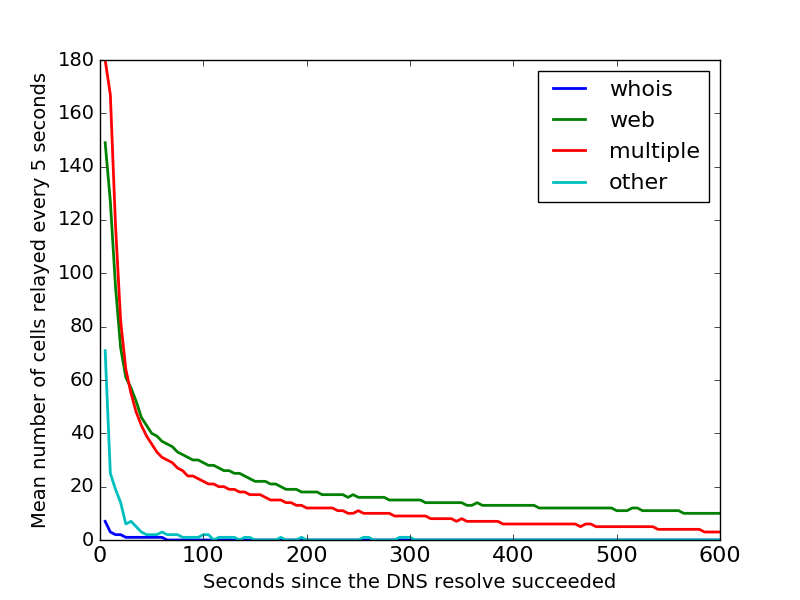
\includegraphics[scale=0.3]{images/exitmeasurement.png}
		\label{fig:stats_a}
		\caption{Time Profile}
	\end{subfigure}
	\begin{subfigure}[t]{0.32\textwidth}
		\centering
		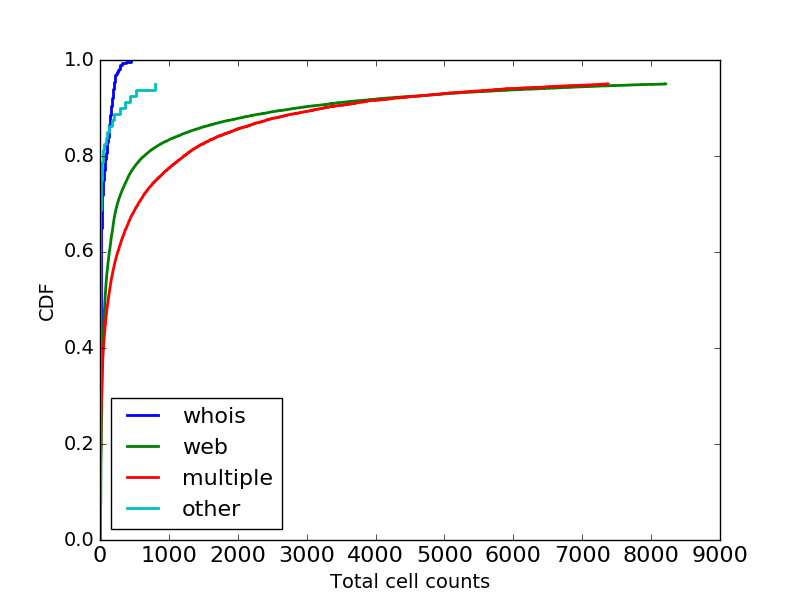
\includegraphics[scale=0.3]{images/totcellcountscdf.png}
		\label{fig:stats_b}
		\caption{Total Counts}
	\end{subfigure}
	\begin{subfigure}[t]{0.32\textwidth}
		\centering
		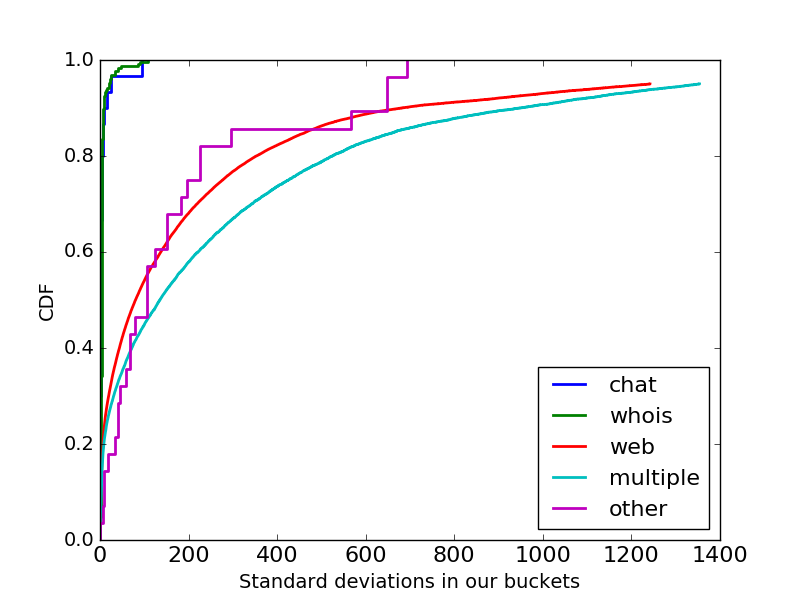
\includegraphics[scale=0.3]{images/stddevs.png}
		\label{fig:stats_c}
		\caption{Time Stdevs}
	\end{subfigure}
	\label{fig:measurements}
	\caption{Tor measurements}
\end{figure*}
